\documentclass[12pt]{report}%\documentclass{report}
\usepackage[a4paper,width=150mm,top=25mm,bottom=25mm]{geometry}
\usepackage[utf8]{vietnam}
\usepackage[utf8]{inputenc}
\usepackage[vietnam]{babel}
\usepackage{biblatex}
\usepackage{amsfonts} 
\usepackage{mathtools}
\usepackage{graphicx}
\usepackage{booktabs}
\usepackage{caption}
\usepackage{chngcntr}
\usepackage{mfirstuc}
\usepackage{hyperref}
\usepackage{indentfirst}

\usepackage{etoolbox}
\makeatletter
\patchcmd{\@caption}{\csname the#1\endcsname}{\csname fnum@#1\endcsname:}{}{}
\renewcommand*\l@figure{\@dottedtocline{1}{1.5em}{4.5em}} % default for 3rd arg: 2.3em
\let\l@table\l@figure % as in article.cls
\makeatother

%\counterwithin{figure}{section}
%\numberwithin{equation}{section}

\usepackage{float}
\floatstyle{plaintop}
\restylefloat{table}
\usepackage{tikz} 

%--------------Define list of some thing ---------%
\usepackage{tocloft} %define some thing your own
\newcommand{\listexamplename}{Thuật ngữ}
\newlistof{word}{wor}{\listexamplename}
\newcommand{\word}[2]{%Số 2 ở đây biểu thị cho số biến truyền vào
    \refstepcounter{word}%
    \textit{#1 (#2)}%
    \addcontentsline{wor}{word}
    {\protect
    \begin{tabular}{p{6.2cm}p{6cm}}
        \MakeLowercase{#1} & \MakeLowercase{#2}\\
    \end{tabular}
    }
}

%\usepackage[top=3.5cm, bottom=3.0cm, left=3.5cm, right=2.0cm]{geometry}
\renewcommand{\baselinestretch}{1.5}

\addbibresource{SingleImageGan.bib}

\let\oldnorm\norm   % <-- Store original \norm as \oldnorm
\let\norm\undefined % <-- "Undefine" \norm
\DeclarePairedDelimiter\norm{\lVert}{\rVert}



\begin{document}

\begin{titlepage}

\begin{tikzpicture}[remember picture,overlay,inner sep=0,outer sep=0]
     \draw[blue!70!black,line width=4pt] ([xshift=-1.5cm,yshift=-2cm]current page.north east) coordinate (A)--([xshift=1.5cm,yshift=-2cm]current page.north west) coordinate(B)--([xshift=1.5cm,yshift=2cm]current page.south west) coordinate (C)--([xshift=-1.5cm,yshift=2cm]current page.south east) coordinate(D)--cycle;

     \draw ([yshift=0.5cm,xshift=-0.5cm]A)-- ([yshift=0.5cm,xshift=0.5cm]B)--
     ([yshift=-0.5cm,xshift=0.5cm]B) --([yshift=-0.5cm,xshift=-0.5cm]B)--([yshift=0.5cm,xshift=-0.5cm]C)--([yshift=0.5cm,xshift=0.5cm]C)--([yshift=-0.5cm,xshift=0.5cm]C)-- ([yshift=-0.5cm,xshift=-0.5cm]D)--([yshift=0.5cm,xshift=-0.5cm]D)--([yshift=0.5cm,xshift=0.5cm]D)--([yshift=-0.5cm,xshift=0.5cm]A)--([yshift=-0.5cm,xshift=-0.5cm]A)--([yshift=0.5cm,xshift=-0.5cm]A);


     \draw ([yshift=-0.3cm,xshift=0.3cm]A)-- ([yshift=-0.3cm,xshift=-0.3cm]B)--
     ([yshift=0.3cm,xshift=-0.3cm]B) --([yshift=0.3cm,xshift=0.3cm]B)--([yshift00=-0.3cm,xshift=0.3cm]C)--([yshift=-0.3cm,xshift=-0.3cm]C)--([yshift=0.3cm,xshift=-0.3cm]C)-- ([yshift=0.3cm,xshift=0.3cm]D)--([yshift=-0.3cm,xshift=0.3cm]D)--([yshift=-0.3cm,xshift=-0.3cm]D)--([yshift=0.3cm,xshift=-0.3cm]A)--([yshift=0.3cm,xshift=0.3cm]A)--([yshift=-0.3cm,xshift=0.3cm]A);

   \end{tikzpicture}
   
\begin{center}
    \textbf{ĐẠI HỌC QUỐC GIA THÀNH PHỐ HỒ CHÍ MINH}
    
    \textbf{TRƯỜNG ĐẠI HỌC KHOA HỌC TỰ NHIÊN}
    
    \textbf{KHOA TOÁN TIN-HỌC}
\end{center}
\vspace{10pt}
\begin{center}
    \includegraphics[scale=0.4]{img/logo-khtn.png}
    
% \begin{comment}
    
    
%     \begin{flushleft}
%     \fontsize{14pt}{17pt}\selectfont  
%     \textbf{\textsl{ĐỀ TÀI}}
% \end{flushleft}

% \end{comment}    
    
    \vspace{15pt}
    \fontsize{15pt}{15pt}\selectfont 
\textit{}    %\textbf{BÁO CÁO} 
\vspace{10pt}
    \textbf{KHÓA LUẬN TỐT NGHIỆP ĐẠI HỌC}
    
\end{center}


\begin{center}
\vspace{5pt}
    \fontsize{20pt}{20pt}\selectfont 
    \textit{}
    \textbf{MULTI-SCALE LEARNING A GAN \\ FROM A SINGLE REPRESENTATIVE}
    %\textbf{\textrm{Multi-scale Learning a GAN \\ from a Single Representative}}
\end{center}
\begin{right}

\vspace{30pt}
\textbf{Thực hiện: SV Lý Phi Long}

\vspace{15pt}
 \\
\textbf{Hướng dẫn: TS. Huỳnh Thế Đăng}



\vspace{100pt}
\end{right}

\begin{center}
    \textbf{Tp. Hồ Chí Minh, 2020}
\end{center}
\end{titlepage}

\thispagestyle{empty}

\clearpage
\chapter*{Lời cảm ơn}
Để hoàn thành tốt đề tài tốt nghiệp này, ngoài sự nỗ lực của bản thân, em  còn nhận được sự quan tâm giúp đỡ của nhiều tập thể và cá nhân.

Đặc biệt, em xin bày tỏ lòng biết ơn sâu sắc đến Thầy hướng dẫn của em, TS. Huỳnh Thế Đăng. Thầy không những hỗ trợ em về mặt chuyên môn cũng như ý tưởng mà còn hướng dẫn em về tư duy nghiên cứu khoa học. Em rất tự hào khi trở thành sinh viên của thầy.

Bên cạnh đó, em xin gửi lời cảm ơn chân thành đến  quý Thầy Cô trong Bộ môn  Ứng dụng Tin học đã tạo môi trường học tập thuận lợi để em có thể hoàn thành  khóa luận này. Đồng thời, em  xin cảm ơn đến quý Thầy Cô trong khoa Toán-Tin học, trường ĐH Khoa học Tự nhiên, ĐHQG-HCM đã dạy bảo em tận tình trong suốt quá trình em học tập tại khoa.

Do thời gian thực hiện khóa luận không nhiều, kiến thức còn hạn chế nên khi làm khóa luận em không tránh khỏi những sai sót. Em mong nhận được sự góp ý từ quý Thầy, Cô và bạn đọc. Xin chân thân cảm ơn!

Cuối cùng, em xin kính chúc quý Thầy, Cô dồi dào sức khỏe và thành công trong sự nghiệp cao quý của mình.

\begin{flushright}
{\it Tp.HCM, ngày 25 tháng 08 năm 2020}

Sinh viên\hskip 2.5cm\quad

\vspace{30pt}
{\bf Lý Phi Long} \hskip 1.9cm \quad\
\end{flushright}


\addcontentsline{toc}{chapter}{Lời cảm ơn}

\clearpage
\chapter*{Tóm tắt}
\addcontentsline{toc}{chapter}{Tóm tắt}
Bài toán \word{từ hình ảnh sang hình ảnh}{image-to-image}(I2I) bằng phương pháp học \word{ không giám sát}{unsupervise learning} từ lâu đã trở thành một ứng dụng không thể thiếu của các phương pháp học sâu. Tuy nhiên, để thực hiện được bài toán trên mô hình cần một lượng dữ liệu nhất định để huấn luyện. Nghiên cứu này được xây dựng dựa trên mô hình ConSinGAN \cite{hinz2020improved} và nghiên cứu của Benaim cùng cộng sự \cite{benaim2020structuralanalogy}  nhằm thực hiện chuyển đổi một video sang một video khác theo dạng của một hình ảnh cho trước,  đưa về bài toán chuyển đổi từ hình ảnh sang hình ảnh và chỉ dùng hai hình ảnh $A$ và $B$ cho quá trình huấn luyện trong thời gian ngắn nhất. Mô hình sẽ học được ánh xạ để chuyển đổi từ tầng thô sơ nhất đến tầng chi tiết nhất ứng với từng độ phân giải khác nhau của hình ảnh. Nhờ đó, hình ảnh sẽ được chuyển đổi từ cấu trúc tổng quát nhất đến những chi tiết nhỏ nhất trong  hình. Tuy nhiên, việc lựa chọn kết hợp hai mô hình \cite{benaim2020structuralanalogy} và \cite{hinz2020improved} đã tạo ra những kết quả không tốt và điều đó trở thành tiền đề nên tránh cho các nghiên cứu sao này. 

\clearpage
%\enlargethispage{10\baselineskip}
\tableofcontents
\clearpage

\listoffigures
\clearpage
\listoftables
\clearpage

\listofword\label{listofword}
\clearpage

\chapter{Mở đầu}
\section{Lý do chọn đề tài}

Ngày nay, các \word{mạng đối sinh}{Generative Adversarial Network}(GAN) đã đạt được  nhiều kết quả nổi bật trong nghiên cứu và cả trong ứng dụng, có thể kể đến như tạo ảnh \cite{DBLP:journals/corr/abs-1804-07455}, xóa những vật thể không mong muốn trong ảnh \cite{IizukaSIGGRAPH2017}, tự động tạo ra một đoạn văn bản \cite{nie2018relgan}, xử lý ảnh y khoa, phân đoạn ảnh, tự động tô màu  ảnh, chuyển đổi ảnh \cite{DBLP:journals/corr/abs-1712-00516} và tạo ảnh nghệ thuật \cite{DBLP:journals/corr/ElgammalLEM17}. Không những thế, GAN còn được ứng dụng  rộng rãi trong việc tổng hợp và chỉnh sửa ảnh  mặt người như đoán số tuổi \cite{DBLP:journals/corr/abs-1711-10352, ZhangSQ17}, chuyển đổi giới tính \cite{Wang_2019}.

Tuy nhiên, để có thể huấn luyện được GAN  cần phải có một số lượng dữ liệu khổng lồ và điều này đã gây bất lợi cho các mô hình học sâu nói chung và GAN nói riêng, nên việc giảm số lượng dữ liệu \word{đầu vào}{input}cho GAN dường như là một trong những hướng nghiên cứu trong tương lai. Vào năm 2019, Shaham cùng nhóm cộng sự \cite{Shaham_2019} đã giới thiệu SinGAN, đây là mô hình GAN có rất nhiều ứng dụng như tạo ảnh vô điều kiện, hòa trộn ảnh, chuyển đổi hình vẽ sang hình thật, tăng độ phân giải, làm chuyển động cho ảnh. Mô hình SinGAN đã đạt được nhiều ứng dụng như vậy nhưng quá trình huấn luyện mô hình chỉ diễn ra trên một tấm ảnh duy nhất, điều này đã tạo nên một bước đệm trong nghiên cứu huấn luyện GAN trên một hình ảnh.
\clearpage
\section{Mục tiêu nghiên cứu}
Vào năm 2020, Hinz cùng cộng sự \cite{hinz2020improved} đã đề xuất mô hình ConSinGAN nhằm cải tiến thời gian huấn luyện SinGAN và Benaim cùng cộng sự \cite{benaim2020structuralanalogy} đã đưa ra những ứng dụng mới cho SinGAN trong đó có ứng dụng chuyển đổi từ video này sang video khác mang kiểu dáng của hình ảnh cho trước. Điều này đã thôi thúc sự ra đời của nghiên cứu này nhằm kết hợp cả hai mô hình trên lại với mong muốn giữ được các đặc tính tốt nhất của các nghiên cứu \cite{benaim2020structuralanalogy, hinz2020improved}.  Cụ thể, các nội dung như sau:
\begin{itemize}
    \item Mô hình sẽ tận dụng sức mạnh của kiến trúc đa tầng  nhằm giải quyết được bài chuyển đổi từ hình ảnh sang hình ảnh.
    \item Bằng cách kết hợp mô hình ConSinGAN \cite{hinz2020improved} và mô hình của Benaim và cộng sự \cite{benaim2020structuralanalogy}, ta có thể mong đợi việc xây dựng mô hình nhằm giải quyết bài toàn chuyển đổi từ hình ảnh sang hình ảnh với mô hình ít tham số nhất.
\end{itemize}

\clearpage

\chapter{Phương pháp nghiên cứu gần đây}
\section{Mạng đối sinh}
\begin{figure*}[t]
\vspace{-0.5cm}
	\centering
	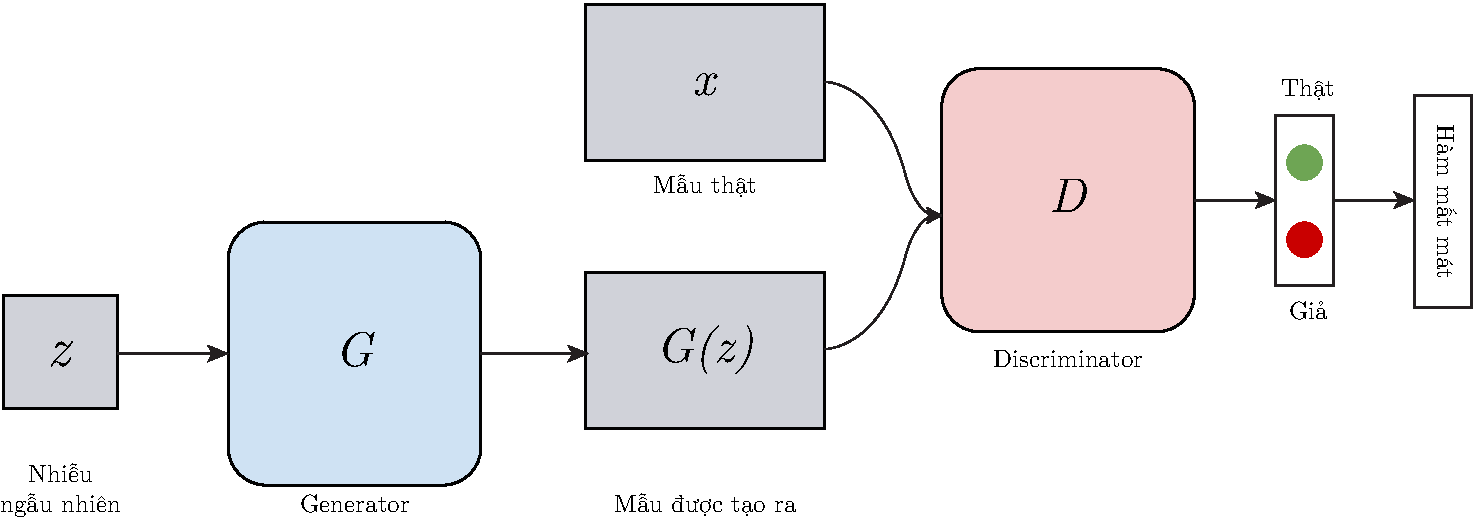
\includegraphics[width=0.85\textwidth]{img/GAN-structure.pdf}
	\caption[Cấu trúc tổng quát của mạng đối sinh]{\blindtext Cấu trúc tổng quát của mạng đối sinh. \quad Đầu vào của $G$ là $z$, với $z$ là nhiễu được khởi tạo ngẫu nhiên. $D$ sẽ lấy mẫu được  sinh ra từ $G$ là $G(z)$ và mẫu thật $x$ từ tập huấn luyện. $D$ sẽ giải quyết bài toán phân loại nhị phân, trả về kết quả từ 0 đến 1, với xác suất đầu ra càng cao thì khả năng mẫu đó là thật càng lớn và ngược lại.}
	\label{fig:architecture} \vspace{-0.4cm}
\end{figure*}

Mạng đối sinh lần đầu tiên được giới thiệu bởi Goodfellow \cite{goodfellow2014generative} và được cấu tạo bởi hai phần: \word{bộ sinh}{generator}(ký hiệu $G$) và \word{bộ phân biệt}{discriminator}(ký hiệu $D$). Cấu trúc tổng quát được miêu tả như hình \ref{fig:architecture}.

Trong đó, $G$ sẽ tạo ra những \word{mẫu}{sample}tương tự với dữ liệu thật, trong khi  $D$ sẽ cố gắng phân biệt đâu là mẫu từ phân phối dữ liệu thật,  đâu là mẫu do   $G$ tạo ra. Có thể tưởng tượng,   $G$ là một nhóm người làm hàng giả, còn   $D$ là cảnh sát cố gắng phát hiện ra được hàng giả. Quá trình huấn luyện diễn ra như một cuộc cạnh tranh  nhằm bắt buộc cả   $G$ và   $D$ cải thiện dần dần phương pháp học  tốt hơn.

$D$ sẽ cho ra giá trị dự đoán $D(x)$ cho biết $x$ có phải là ảnh thật hay không. Mục tiêu của   $D$ là tối đa hóa khả năng phân biệt được hình ảnh nào là hình ảnh thật và  hình ảnh nào là hình ảnh do   $G$ tạo ra.   $D$ sẽ được huấn luyện để giá trị $D\left( x \right) \rightarrow 1$ còn $D\left( G\left(x \right) \right) \rightarrow 0$. Nghĩa là, \word{hàm mất mát}{loss function}muốn tối đa hóa giá trị $D\left(x\right)$ và tối thiểu hóa giá trị $D\left(G\left(x\right)\right)$. Quá trình tối thiểu hóa  giá trị $D\left(G\left(x\right)\right)$ tương đương với việc tối đa hóa $\left(1 - D\left(G\left(x\right)\right)\right)$. Vì vậy, hàm mất mát của  $D$ là:
\begin{equation}\label{D-loss}
    \mathop {\max }\limits_D V\left( {D} \right) = {{\rm \mathbb{E}}_{x \sim p_{data}\left( x \right)}}\left[ {\log D\left( x \right)} \right] + {{\rm \mathbb{E}}_{z \sim p_z\left( z \right)}}\left[ {\log \left( {1 - D\left( {G\left( z \right)} \right)} \right)} \right]
\end{equation}
Trong đó, $p_{data}(x)$ là ký hiệu cho phân phối dữ liệu thật, $p_z(z)$ là  ký hiệu cho phân phối nhiễu.

$G$ sẽ học cách đánh lừa   $D$ bằng cách sinh ra ảnh gần giống thật, hay giá trị $D\left(G\left(x\right)\right) \rightarrow 1$. Tức là, hàm mất mát mong muốn tối đa hóa giá trị $D\left(G\left(x\right)\right)$, tương đương với việc tối thiểu hóa giá trị  $\left(1 - D\left(G\left(x\right)\right)\right)$. Vì vậy, hàm mất mát của   $G$ là:
\begin{equation}\label{G-loss}
    \mathop {\min }\limits_G  V\left( {G} \right) = {{\rm \mathbb{E}}_{z \sim p_z\left( z \right)}}\left[ {\log \left( {1 - D\left( {G\left( z \right)} \right)} \right)} \right]
\end{equation}
Do đó, hàm mất mát tổng quát của GAN được định nghĩa:
\begin{equation}\label{GAN-loss}
    \mathop {\min }\limits_G \mathop {\max }\limits_D V\left( {D,G} \right) = {{\rm \mathbb{E}}_{x \sim p_{data}\left( x \right)}}\left[ {\log D\left( x \right)} \right] + {{\rm \mathbb{E}}_{z \sim p_z\left( z \right)}}\left[ {\log \left( {1 - D\left( {G\left( z \right)} \right)} \right)} \right]
\end{equation}
Từ hàm mất mát của GAN, ta có thể thấy là quá trình huấn luyện    $G$ và   $D$ là quá trình đối nghịch nhau, trong khi $D$ cố gắng tối đa hóa hàm mất mát thì $G$ cố gắng tối thiểu hóa hàm mất mát. Quá trình huấn luyện GAN kết thúc khi GAN đạt đến trạng thái cân bằng của cả hai mô hình $G$ và $D$, được gọi là \word{cân bằng Nash}{Nash Equilibrium}.

\clearpage
\section{Mô hình sinh được huấn luyện trên một ảnh}
%Cần bổ sung thêm
Quá trình huấn luyện để học được phân phối của các \word{vùng nhỏ}{patch}trên một tấm ảnh từ lâu đã được chứng minh rất tốt.
Bằng hướng tiếp cận này, mà nhiều bài toán  như \word{nội suy ảnh}{inpainting} \cite{Ulyanov2018DeepIP,Zhang_2019}, \word{khử nhiễu}{denoise} \cite{Zontak2013SeparatingSF}, \word{siêu phân giải}{super-resolution} \cite{Michaeli2014BlindDU}, \word{phân đoạn ảnh}{image segmentation} \cite{Gandelsman2019DoubleDIPUI} đã được giải quyết mà chỉ cần huấn luyện một hình ảnh duy nhất. Cụ thể, bài toán siêu phân giải hình ảnh \cite{Yang2019DeepLF, Huang_2015_CVPR, Glasner2009SuperresolutionFA, BellKligler2019BlindSK} và chỉnh sửa hình ảnh \cite{Cho2008ThePT,mechrez2016saliency, Tlusty2018ModifyingNV} đã được tập trung vào nghiên cứu theo hướng huấn luyện bằng một ảnh duy nhất và đã đạt được kết quả tốt. Hơn nữa, vài nghiên cứu gần đây cũng chỉ ra việc sử dụng một tấm ảnh cũng đủ thông tin để giúp huấn luyện mô hình \cite{YM.2020A}.

Tuy nhiên, các nghiên cứu về huấn luyện GAN trên tấm ảnh duy nhất vẫn còn chưa nhiều. Hầu hết, các mô hình này đều không sử dụng hình ảnh "tự nhiên", mà thay vào đó họ chỉ huấn luyện mô hình học các thông tin họa tiết trên hình \cite{jetchev2016texture, zhou2018non, bergmann2017learning, li2016precomputed}. Trong thời gian gần đây, hai mô hình GAN đã được đề xuất mà quá huấn luyện chỉ diễn ra trên một  hình ảnh "tự nhiên", cụ thể là InGAN \cite{shocher2018zero} và SinGAN \cite{Shaham_2019}. Bên cạnh đó, còn có mô hình ConSinGAN \cite{hinz2020improved} nhằm cải tiến mô hình SinGAN để giúp việc huấn luyện trở nên dễ dàng và nhanh hơn. 

SinGAN xây dựng kiến trúc mô hình như một kim tự tháp nhằm huấn luyện cả bộ sinh và bộ phân biệt qua nhiều tầng, mỗi tầng ứng với một độ phân giải khác nhau của  hình ảnh. Tại mỗi tầng, mô hình được huấn luyện riêng biệt và \word{trọng số}{weight}của mô hình ở các tầng phía trước sẽ được giữ cố định. \word{Đầu ra}{output}của mỗi tầng là một hình ảnh và hình ảnh đó sẽ được \word{tăng mẫu}{upsamling} theo hệ số $r^s \left(r,s \in \mathbb{R} \right)$ và trở thành đầu vào cho tầng tiếp theo. Mô hình ConSinGAN cũng sử dụng cấu trúc tương tự như SinGAN, tuy nhiên thay vì huấn luyện mỗi tầng là độc lập, thì  ConSinGAN sẽ huấn luyện $3$ tầng với nhau để đạt được kết quả tốt hơn. Trong nghiên cứu này, mô hình   sẽ được xây dựng dựa trên  ConSinGAN \cite{hinz2020improved} và nghiên cứu của Benaim cùng cộng sự \cite{benaim2020structuralanalogy}.
\clearpage
\section{Bài toán chuyển đổi hình ảnh sang hình ảnh}

Bài toán chuyển đổi hình ảnh sang hình ảnh là bài toán rất phổ biến trong GAN với mục tiêu giúp  mô hình học được ánh xạ giữa ảnh đầu vào và ảnh đầu ra \cite{hertzmann2001image}. Nhờ sự phát triển mạnh mẽ của mạng học sâu mà các mạng đối sinh đã đạt nhiều kết quả khá tốt trong bài toán I2I. Isola cùng với các cộng sự \cite{isola2017image} đã đề xuất mô hình "pix2pix" - mạng GAN có điều kiện - nhằm thực hiện một số ứng dụng trong bài toán I2I theo phương pháp \word{học giám sát}{supervise learning}, tức là dữ liệu sẽ được đi theo từng đôi. Tuy nhiên, việc tìm dữ liệu theo từng đôi là rất khó, thậm chí là bất khả thi trong một số trường hợp. Ví dụ, việc chuyển đổi qua lại giữa hình ảnh đời thường và hình ảnh do các nghệ sỹ vẽ. Các mô hình  DiscoGAN \cite{kim2017learning}, CycleGAN \cite{zhu2017unpaired} và DualGAN \cite{yi2017dualgan} đã được đề xuất nhằm giải quyết bài toán I2I với phương pháp  học không giám sát bằng cách sử dụng  \word{mất mát chu kỳ nhất quán}{cycle-consistent loss}. Liu cùng  cộng sự \cite{liu2019fewshot} đề xuất mô hình FUNIT có thể chuyển đổi được nhiều miền ảnh hơn. Tuy nhiên, FUNIT cần rất nhiều dữ liệu để huấn luyện, đồng thời dữ liệu giữa hai miền cũng phải tương tự nhau. Trong nghiên cứu này không cần bất kỳ một \word{mô hình tiền huấn luyện}{pre-train model}nào cũng như không cần bất kỳ một yêu cầu đặc biệt nào về dữ liệu, trong đó  bao gồm việc sử dụng hình ảnh "tự nhiên", từ một video và một hình ảnh làm gốc, sẽ chuyển đổi thành một video khác mang kiểu dáng giống như hình ảnh đó.

\clearpage
\chapter{Phương pháp nghiên cứu đề xuất}
\label{our-method}
Đầu vào của bài toán là một video và hình ảnh mục tiêu. Mô hình sẽ chuyển đổi video đầu vào thành video đầu ra có kiểu dáng giống \word{hình ảnh mục tiêu}{target image}. Video đầu vào gồm chuỗi các khung hình $f_0, f_1,...,f_k$ với $k\in \matbb{N}$. Do đó, tại mỗi vòng lặp, ta sẽ chọn ngẫu nhiên một khung hình $f_i$ bất kỳ làm hình ảnh gốc $I_A$ và hình ảnh mục tiêu đặt là $I_B$. Điều này đã đưa bài toán đang làm thành bài toán chuyển đổi hai hình ảnh  $I_A \in A$ và $I_B \in B$, trong đó $A$ và $B$ là hai miền ảnh tương ứng, bằng cách chuyển đổi $I_A$ sang $I_{AB} \in B$ và $I_B$ sang $I_{BA} \in A$ mà không cần bất kỳ dữ liệu nào khác. Như được đề cập ở trên, dữ liệu đầu vào rất hạn chế, nên mô hình sẽ huấn luyện $G_A$ và $G_B$ qua nhiều tầng, từ tầng thô sơ nhất đến chi tiết nhất.
Ban đầu, mô hình tiến hành \word{giảm mẫu}{downsample} $I_A$ và $I_B$ thành hai kim tự tháp gồm $N$ tầng ($N \in \mathbb{N}$): $\mathcal{I}_A = \left\{ I_A ^n | n = 0,1,...,N-1\right\}$ và $\mathcal{I}_B = \left\{ I_B ^n | n = 0,1,...,N-1\right\}$.

Các nghiên cứu trước đây cho thấy được sức mạnh của kiến trúc đa tầng trong việc tạo ảnh vô điều kiện \cite{karras2017progressive, huang2017stacked, denton2015deep}, tạo ảnh điều kiện \cite{wang2017high} hay dùng để huấn luyện mô hình bằng một ảnh \cite{Shaham_2019, hinz2020improved}. Trong nghiên cứu này sẽ tận dụng kiến trúc đa tầng vào ứng dụng chuyển đổi hình ảnh không giám sát như trong nghiên cứu của Benaim cùng cộng sự \cite{benaim2020structuralanalogy}  và đồng thời sử dụng các cải tiến của mô hình ConSinGAN \cite{hinz2020improved} cho SinGAN \cite{Shaham_2019} với hy vọng đạt được mong muốn có thể giữ được các đặc điểm tốt của mô hình mà vẫn có thể giải được bài toán.

\section{Kiến trúc mô hình}
Kiến trúc của mô hình được minh họa trong hình \ref{fig:model-structure} (a). Trong đó, $G_A$ và $G_B$ là chuỗi các bộ sinh, $\left\{ G_A ^n\right\}_{n=0} ^N$ và $\left\{ G_B ^n \right\}_{n=0} ^N$ được dùng để chuyển đổi hình ảnh ứng với tầng $n$. Tại mỗi tầng,  ta cần có hai bộ phân biệt $D_A ^n$ và $D_B ^n$ $\left( n \in \left\{ 0,1,...,N\right\}\right)$ được dùng để phân biệt hình ảnh đầu vào có phải là hình ảnh thật trong miền $A$ và $B$ hay không. Kiến trúc của mô hình được chia làm hai phần chính: Trình tạo ảnh vô điều kiện và trình tạo ảnh điều kiện. 
\begin{figure*}[p]
\vspace{-0.5cm}
	\centering
	\includegraphics[width=1\textwidth]{img/sturcture-compare_2.pdf}
	\caption[So sánh kiến trúc hai mô hình]{\blindtext So sánh kiến trúc hai mô hình. \quad Hình vẽ miêu tả quá trình chuyển đổi từ ngọn lửa sang vịt đá trong mô hình nghiên cứu này và mô hình của Benaim cùng cộng sự. Trong đó, $I_A ^n$ là hình ảnh ngọn lửa, $I_B ^n$ là hình ảnh vịt đá tại tầng $n$ với $0<n<N$. Đầu tiên đối với cả hai mô hình, bộ sinh $G_A ^n$ tạo ra hình ảnh ngọn lửa giả tại tầng $n$, bằng cách đưa vào nhiễu ngẫu nhiên $z_n$ được khởi tạo theo phân phối Gaussian. Sau đó,  $D_A ^n$ được dùng để phân biệt $\overline{I}_A ^n$ với hình ảnh gốc $I_A ^n$. Bộ sinh $G_B ^n$ sẽ ánh xạ $\overline{I}_A ^n$ thành $\overline{I}_{AB} ^n$ . Khi đó, $D_B ^n$ sẽ phân biệt $\overline{I}_{AB} ^n$ với hình ảnh gốc $I_B ^n$. Bộ sinh $G_A ^n$ tiếp tục ánh xạ $\overline{I}_{AB} ^n$ sang $\overline{I}_{ABA} ^n$ để chắc chắn khoảng cách giữa $\overline{I}_{ABA} ^n$ và $\overline{I}_{A} ^n$ gần nhau. Hình (a) là kiến trúc của mô hình được xây dựng trong nghiên cứu này: Đầu vào ở các tầng là đặc trưng được trích xuất từ tầng trước. Hình (b) là kiến trúc được đề xuất bởi Benaim \cite{benaim2020structuralanalogy}: Đầu vào ở các tầng tiếp theo sẽ  là hình ảnh được nâng độ phân giải ở tầng trước được thêm nhiễu.}
	\label{fig:model-structure} \vspace{-0.4cm}
\end{figure*}
\subsection{Kiến trúc đa tầng}

\textbf{Trình tạo ảnh vô điều kiện} \quad 
Tại bất kỳ tầng $n$, để tìm ánh xạ giữa hai miền $A$ và $B$, đầu tiên, mô hình sẽ giảm mẫu	 hình ảnh $I_A$ và $I_B$ xuống thành $I_A ^n$ và $I_B ^n$ theo một hệ số $r^s \left(r,s \in \mathbb{R} \right)$ (xem phần \ref{resize}).

% What: Thay đổi cách truyền dữ liệu
Tương tự mô hình của Benaim cùng cộng sự, mô hình cũng sẽ được huấn luyện từ tầng thô sơ nhất đến tầng tốt nhất. Sau đó, được huấn luyên xuyên suốt qua các tầng từ đầu đến cuối thay vì chỉ huấn luyện độc lập các tầng với nhau.Khác với, nghiên cứu của Benaim cùng cộng sự là mô hình chỉ được huấn luyện tại tầng hiện tại (cao nhất) và các tham số của tất cả các tầng phía trước sẽ được đóng băng. Tuy nhiên, mô hình trong nghiên cứu này sẽ không huấn luyện xuyên suốt qua các tầng vì sẽ rất dễ dẫn đến hiện tượng \word{quá khớp}{overfiting} nên mô hình sẽ được huấn luyện từng tầng một và các tham số của tầng trước đó sẽ không bị đóng băng. 

Tại tầng thô sơ nhất $n=0$, cả mô hình của Benaim cùng với cộng sự và mô hình trong nghiên cứu này đều sẽ học được ánh xạ từ nhiễu $z$ đến hình ảnh có độ phân giải thấp nhất:
\begin{equation}\label{fake_A_uncondition_0}
    \overline I _A^0 = G_A^0\left( {z_A^0} \right)    
\end{equation}
\begin{equation}\label{fake_B_uncondition_0}
    \overline I _B^0 = G_B^0\left( {z_B^0} \right)
\end{equation}
Trong đó, $z_A ^n$ là nhiễu được khởi tạo theo chuẩn Gaussian.

Khi lên tầng cao hơn $n>0$, mô hình của Benaim và cộng sự sẽ đưa hình ảnh được tạo ra ở tầng trước được \word{nâng độ phân giải}{upscale}và cộng thêm vào nhiễu $z_n$ để đưa đến tầng tiếp theo:
\begin{equation}\label{fake_A_uncondition_bea}
    \overline I _A^n = G_A^n\left( {z_A^n} + \uparrow{\overline{I}_A ^ {n-1}}\right)    
\end{equation}
\begin{equation}\label{fake_B_uncondition_bea}
    \overline I _B^n = G_B^n\left( {z_B^0} + \uparrow{\overline{I}_B ^ {n-1}}\right)
\end{equation}

Khác với mô hình Benaim cùng cộng sự, khi lên tầng cao hơn $n>0$,  thay vì mô hình nhận đầu vào là hình ảnh được nâng độ phân giải  từ tầng trước thì  trong nghiên cứu này mô  sẽ nhận đầu vào là các \word{đặc trưng}{feature}được trích xuất ra từ tầng trước và  truyền vào tầng tiếp theo. Đồng thời, nhiễu  cũng sẽ đươc thêm ở tất cả các tầng của mô hình:%Why: Tại sao phải thay đổi như vậy?
\begin{equation}\label{fake_A_uncondition}
    \overline I _A^n = G_A^n\left( {z_A^n} + G_A^{n-1}\left( z_A ^{n-1} \right)\right)    
\end{equation}
\begin{equation}\label{fake_B_uncondition}
    \overline I _B^n = G_B^n\left( {z_B^n} + G_B^{n-1}\left( z_B ^{n-1} \right)\right)
\end{equation}

Việc truyền trực tiếp đặc trưng được trích xuất ra từ tầng trước giúp cho mô hình tiết kiệm được thời gian huấn luyện, đồng thời sẽ không tốn nhiều chi phí tính toán để huấn luyện lại các tầng trước giống như mô hình của Benaim cùng cộng sự.

% Việc thay đổi này tạo ra kết quả như thế nào?

\textbf{Trình tạo ảnh điều kiện} \quad Tại bất kỳ tầng $n$, kiến trúc đa tầng cả hai mô hình như nhau, đầu vào là  một mẫu $\overline{I}_A ^n \in A$ và $\overline{I}_B ^n \in B$ trong trình tạo ảnh vô điều kiện. Quá trình chuyển đổi hình ảnh sẽ được đi từ tầng thô sơ nhất đến tầng chi tiết nhất. Hai bộ sinh $G_B ^n$ và $G_A ^n$ sẽ ánh xạ $\overline I _A^n$ và $\overline I _B^n$ sang miền ảnh mục tiêu tương ứng. Có thể hiểu một cách toán học như sau: 
\begin{equation}\label{mix_g_b}
    \overline I _{AB}^n = G_B^n\left( {\overline I _A^n} \right)
\end{equation}
\begin{equation}\label{mix_g_a}
    \overline I _{BA}^n = G_A^n\left( {\overline I _B^n} \right)
\end{equation}

Bộ sinh được xem là chuyển đổi tốt khi và chỉ khi đối với mỗi tầng, từng vùng trong ảnh $I_A$ được chuyển đổi tương ứng sang từng vùng trong ảnh $I_B$ và ngược lại. Do đó, tại tầng thô sơ nhất $n=0$, ánh xạ giữa hai hình ảnh $I_A ^0$ và $I_B ^0$ nên ánh xạ được cấu trúc tổng quát nhất từ $I_A$ sang $I_B$. Ví dụ, mặt đất nằm ở phía đáy của hình $I_A$ nên được ánh xạ sang mặt cỏ ở dưới đáy của hình $I_B$, ánh sáng ban ngày trong $I_A$ nên được ánh xạ sang ánh sáng ban đêm bên $I_B$. Đối với những tầng cao hơn $n>0$, bộ sinh $G_B ^n$ và $G_A ^n$ sẽ học được những chi tiết nhỏ hơn trong tấm hình $I_B ^n$ và $I_A ^n$. Tuy nhiên, ánh xạ mà bộ sinh $G_B ^n$ và $G_A ^n$ học được vẫn phải giữ được cấu trúc tổng thể được học từ các tầng trước. 
%bộ sinh $G_B ^n$ nên ánh xạ những chi tiết nhỏ hơn như là kiểu dáng, kết cấu của tấm hình $a$ sang chi tiết trong $b$.


%Ta có thể thấy được tầm quan trọng của kiến trúc đa quy mô trong việc tạo ảnh. Tuy nhiên, có rất nhiều cách để có thể tiếp cận với mô hình đa tầng, ví dụ SinGAN chi huấn luyện tại tầng cao nhất, tất cả các tầng trước sẽ được đóng băng lại không huấn luyện. Mô hình PGGAN [] đưa ra một cách huấn luyện với mô hình đa tầng bằng cách thêm từng tầng vào và không đóng băng các trọng số ỡ tầng trước. 
%Huấn luyện mô hình ConSinGAN bắt đầu từ tầng có hình ảnh thô nhất, mô hình sẽ cố gắng học cách ánh xạ từ nhiễu bất kỳ $z$ thành một hình ảnh có độ phân giải thấp. Khi huấn luyện hết một tầng, chúng tôi sẽ tiến hành tăng kích thước của bộ sinh bằng cách thêm 3 lớp tích chập vào bộ sinh. Chúng tôi lặp lại quá trình này $N$ lần cho tới khi đạt được độ phân giải mong muốn.
\clearpage
\subsection{Cấu trúc bộ sinh} %\quad %Ta sẽ huấn luyện mô hình bắt đầu từ tầng thô sơ nhất để có thể học được ánh xạ từ vecotr nhiễu $z$ đến hình ảnh có độ phân giải thấp (như "bộ sinh: Tầng 0" tronh hình 1).
\begin{figure*}[h]
\vspace{-0.5cm}
	\centering
	\includegraphics[width=1\textwidth]{img/Model_generator (2).pdf}
	\caption[So sánh kiến trúc bộ sinh của hai mô hình]{\blindtext So sánh kiến trúc bộ sinh của hai mô hình. \quad Hình (a) là kiến trúc của mô hình trong nghiên cứu này. Tại mỗi tầng sẽ được thêm mới vào 1 lớp tăng mẫu và 3 khối tích chập. Đồng thời, đầu vào của mỗi tầng là đặc trưng được trích xuất từ tầng trước được cộng thêm nhiễu. Hình (b) là kiến trúc bộ sinh của mô hình Benaim và cộng sự \cite{benaim2020structuralanalogy} gồm 5 khối tích chập. Đồng thời, đầu vào của mỗi tầng là hình ảnh từ tầng trước được nâng độ phân giải và cộng thêm vào nhiễu.}
	\label{fig:generator} \vspace{-0.4cm}
\end{figure*}
%What: Thay đổi cái gì?
Tương tự như SinGAN, cấu trúc bộ sinh của  mô hình Benaim và cộng sự sẽ là một mạng tích chập gồm 5 khối tích chập. Ban đầu mỗi khối tích chập gồm 32 \word{nhân}{kernel}có kích thước ($3 \times 3$)  nối đến một lớp \word{chuẩn hóa theo cụm dữ liệu}{batch norm} và cuối cùng cho đi qua một \word{hàm kích hoạt}{activation function} LeakyReLU như hình \ref{fig:generator} (b). Đầu tiên tại tầng thô sơ nhất $n=0$, nhóm tác giả bắt đầu với 32 nhân  tại mỗi khối và sẽ được tăng số lượng nhân lên gấp đôi sau 4 tầng và số lượng lớp sẽ được giữ nguyên xuyên suốt các tầng.

%What: thay đổi cái gì?
Trong nghiên cứu này, cấu trúc của bộ sinh là một mạng nơ-ron tích chập được miêu tả như hình \ref{fig:generator} (a). Khác biệt với mô hình của Benaim cùng cộng sự, mô hình bộ sinh trong nghiên cứu này được lấy ý tưởng từ mô hình bộ sinh trong PGGAN \cite{karras2017progressive}. Cụ thể, tại tầng thô sơ nhất $n=0$, bộ sinh gồm  3 khối tích chập, mỗi khối tích chập sẽ 64 nhân kích thước ($3 \times 3$) lớp tích chập sau đó sẽ được đi qua hàm kích hoạt Leaky ReLU. Sau khi huấn luyện xong tầng đầu tiên, bộ sinh sẽ được thêm vào 1 lớp tăng mẫu và 3 khối tích chập.  Đặc biệt, đối với các tầng $n>0$, bộ sinh sẽ được thêm vào \word{liên kết dư}{residual connection} từ đặc trưng gốc được tăng mẫu đến đầu ra của lớp tích chập mới được thêm vào  (xem "bộ sinh: Tầng 1" trong hình \ref{fig:generator}). Cũng giống như mô hình của Benaim cùng cộng sự, tại mỗi tầng $n>0$, trước khi thêm vào 3 khối tích chập, đặc trưng gốc từng tầng trước sẽ được thêm vào nhiễu nhằm tạo được độ đa dạng của hình ảnh. Quá trình này sẽ lặp đi lặp lại đến khi nào bộ sinh tạo ra được hình ảnh có độ phân giải như ban đầu. 
%Why: Tại sao lại thay đổi cấu trúc bộ sinh như vậy? Ý đồ đen tối đằng sau là gì
Vì với những tầng có độ phân giải càng nhỏ thì mô hình không cần quá nhiều lớp tích chập để có thể học được các đặc trưng của tấm hình. Đồng thời, điều này giúp giảm được số lượng trọng số của mô hình giúp cho mô hình được huấn luyện nhanh hơn.

%How: Sau khi thay đổi như vậy thì điều kỳ diệu gì sẽ xảy ra? Điều kỳ diệu đó so với bài cũ của người ta nó như thế nào? Tốt hơn tệ hơn?

%Ban đầu, bộ sinh chỉ gồm 1 khối (ba lớp tích chập $3\times3$ xếp chồng lên nhau), sau khi ta huấn luyện xong tầng đầu tiên, ta sẽ tiến thành thêm vào một lớp Upslamping và 1 block (gồm 3 lớp tích chập  $3\times3$ xếp chồng lên nhau). Khác biệt với SinGAN, tại mỗi tầng sẽ lấy đặc trưng gốc từ tầng trước làm đầu vào, và trọng số của layers phía trước sẽ không cố định lại. Ta sẽ thêm vào residual connection từ feature gốc được upsampled đến output của convolutiona layer mới được thêm vào (như "bộ sinh: Tầng 1" trong hình 1). Ta sẽ lặp lại quá trình này $N$ lần đến khi nào ta đạt được độ phân giải đầu ra. 
%Nói thêm về việc huấn luyện 3 tầng
%CŨng giống như SinGAN, ta cũng thêm nhiễu vào từng tầng để có thể cải thiện được độ đa dạng của hình ảnh. Trong cài đặt mặc định, ta sẽ train ít nhất 3 tầng 1 lúc, điều nay có nghĩa 3 khối cuối cùng của 3 lớp convolutional layers. Mô hình có thể huấn luyện một lúc nhiều hơn 3 tầng, tuy nhiên làm như thể sẽ dễ dấn đến mô hình bị overfiting (hình 4)

%Cần ghi nhiều hơn
\subsection{Cấu trúc bộ phân biệt}
Tương tự như mô hình của  Benaim cùng với cộng sự,  bộ phân biệt được sử dụng trong nghiên cứu này là một bộ phân biệt đã được đề xuất trong PatchGAN \cite{isola2017image} gồm 5 khối tích chập, mỗi khối tích chập sẽ có dạng 1 lớp tích chập ($3\times 3$) và hàm kích hoạt Leaky-ReLU.  Bộ phân biệt truyền thống sẽ nhận đầu vào là một hình ảnh và đầu ra là một giá trị xác suất để xem ảnh đầu vào là thật hay giả. Đối với PatchGAN, bộ phân biệt  cũng sẽ nhận hình ảnh làm đầu vào nhưng thay vì đầu ra là một giá trị duy nhất thì đầu ra sẽ là một ma trận $X$ với từng phần tử $X_{ij}$ là kết quả xác suất trên từng vùng ảnh nhỏ của hình ảnh lớn được đưa qua bộ phân biệt.

Bộ phân biệt PatchGAN sẽ phân loại từng vùng nhỏ trên tấm ảnh thay vì trên toàn bộ ảnh nên sẽ có kết quả tốt hơn. Tất nhiên khi huấn luyện bộ phân biệt của PatchGAN với ảnh thật mô hình mong muốn đầu ra của tất cả các vùng ảnh là 1, còn giá trị đầu ra trên tất cả các vùng ảnh giả sẽ là 0. Ngược lại, khi huấn luyện bộ sinh, giá trị mà bộ phân biệt nên trả ra  trên tất các vùng ảnh là 1.

\subsection{Kiến trúc đa tầng cho hình ảnh} 
\label{resize}
Trong xây dựng kiến trúc đa tầng, có một thông số rất quan trọng được dùng để tạo ra kim tự tháp, đó chính là hệ số giảm mẫu hình ảnh. Mô hình của  Benaim cùng  cộng sự cũng sử dụng phương pháp giảm mẫu hình ảnh $x$ tương tự như SinGAN  bằng phép nhân với hệ số  $r^{N-n}$ với $N$ là tổng số lượng tầng của mô hình, $n$ là tầng hiện tại, $r$ là hệ số thay đổi với  giá trị $r$ mặc định là $0.75$. Với cách trên, mô hình phải mất từ 8 đến 10 tầng mới có thể đạt được ảnh có chiều dài hoặc chiều rộng là 250px. Nếu thay đổi giá trị $r$ (ví dụ như $r=0.50$) để giúp việc giảm mẫu diễn ra nhanh hơn, dùng ít tầng hơn thì dẫn đến việc hình ảnh được tạo ra sẽ mất đi cấu trúc tổng quát của chúng.

Trong trường hợp mô hình không đủ tầng để huấn luyện với hình ảnh có độ phân giải thấp thì khi lên những tầng cao hơn, mô hình sẽ không giữ được cấu trúc tổng thể của hình ảnh mà thay vào đó mô hình chỉ có thể học được các thông tin về hoa văn. Do đó, để hình ảnh đạt được bố cục tổng thể  mô hình cần được huấn luyện  đủ lâu ở các tầng mà  hình ảnh có độ phân giải thấp và  không cần quá nhiều tầng với hình ảnh có độ phân giải cao. Vì vậy, phương pháp thay đổi đổi kích thước hình ảnh có thể điều chỉnh để hình ảnh không bị biến đổi hình học quá thô cứng ($x_n = x_N \times r^{N-n}$) và đồng thời giúp cho mô hình trong nghiên cứu này có thể học được đủ lâu ở các tầng hình ảnh  có độ phân giải thấp nhằm giúp cho hình ảnh tạo ra vẫn giữa được cấu trúc tổng quát như ban đầu:
\begin{equation}\label{resize_equal}
    {x_n} = {x_N} \times {r^{\frac{{N - 1}}{{\log \left( N \right)}} \times \log \left( {N - n} \right) + 1}} \textrm{với }  n = 0,1,...N - 1
    \end{equation}
Trong đó,  $r = {\left( {\frac{{25}}{{\min (H,W)}}} \right)^{\frac{1}{{N - 1}}}}$ (với $H,W$ lần lượt là chiều cao và chiều ngang của ảnh đầu vào), $N$ là tầng cao nhất, $n$ là tầng hiện tại, $x_N$ là kích thước ban đầu của  ảnh.

Ví dụ, phương pháp thay đối kích thước trong mô hình của  Benaim cùng cộng sự với hệ số $r = 0.67$  lên hình ảnh có độ phân giải ban đầu là $188 \times 250$px  sẽ tạo ra một cấu trúc đa tầng gồm 6 tầng với độ phân giải tương ứng là  $25\times34\text{px},38\times 50\text{px}, 57 \times 75\text{px}, 84 \times112\text{px}, 126 \times 167\text{px}, 188 \times 250\text{px}$. Tuy nhiên, với hệ số thay đổi 
 $r=0.67$ khi sử dụng phương pháp đề xuất ở phương trình \ref{resize_equal} thì mô hình cũng sẽ được huấn luyện với 6 tầng nhưng  độ phân giải tương ứng là $25 \times 34\text{px}, 32 \times 42\text{px}, 42 \times 56\text{px}, 63 \times 84\text{px}, 126 \times 167\text{px}, 188 \times 250\text{px}$. Có thể thấy được độ phân giải thấp của hình ảnh được tạo ra với phương trình \ref{resize_equal} có mật độ dày hơn phương pháp thay đổi hình ảnh gốc.

%\subsubsection{Tốc độ học tại từng tầng}
%Trong quá trình huấn luyện, tốc độ học đóng vai trò rất lớn, nó ảnh hướng rất nhiều đến chất lượng hình ảnh được tạo ra. Tại bất kỳ một tầng $n$,  thay vì ta sử dụng cùng một tốc độ học cho tất cả các tầng $\left( n, n-1, n -2, ... \right)$ thì ta dùng tốc độ học nhỏ hơn cho những tầng thấp hơn  $\left(  n-1, n -2, ... \right)$ sẽ giúp ta giảm được hiện tượng quá khớp (overfiting). Nếu như ta huấn luyện với tốc độ học quá lớn, mô hình sẽ bị sụp đổ (model collapse) và chỉ có thể tạo được hình ảnh giống với hình ảnh đã học. Do đó, ta sẽ thay đổi tốc độ học $\eta$ với hệ số $\delta$. Điều này có nghĩa là, tại mỗi tầng $n$, ta sẽ huấn luyện với tốc độ học là ${\delta}\eta $. Ví dụ, tầng thứ $n-1$ sẽ được huấn luyện với tốc độ học ${\delta ^1}\eta $ tầng thứ $n-2$ sẽ huấn luyện với tốc độ học ${\delta ^2}\eta $. Trong bài này, ta thấy được là $\delta  = 0.1$ là điểm cân bằng giữa chất lượng hình ảnh và độ đa dạng của hình ảnh tạo ra.
\clearpage

\section{Hàm mất mát}
\subsection{Mất mát đối kháng} 
%Nhằm đảm bảo  ${\overline I _A ^n}$ thuộc về phân phối $p_A^n$ và ${\overline {ab} _n}$ thuộc về phân phối $p_B^n$, chúng tôi sử dụng hàm học đối kháng trên từng phần bằng markov bộ phân biệt $D_A ^n$. Kiến trúc của bộ phân biệt $D$ là một mạng nơ-ron tích chập có kiến trúc như hình . 
\word{Mất mát đối kháng}{Adversarial loss} được xây dựng nhằm để bộ phân biệt cố gắng phân biệt được hình ảnh thật từ hình ảnh tổng hợp được trong khi đó bộ sinh sẽ cố gắng đánh lừa bộ phân biệt bằng cách tạo ra ảnh giống thật nhất. Tại tầng thứ $n$, hai bộ phân biệt sẽ nhận được hình ảnh làm đầu vào. Đầu ra sẽ là điểm đánh giá của hình ảnh đầu vào là thật hay giả so với từng miền hình ảnh tương ứng. Cụ thể tại tầng $n$,  $D_A ^n$ sẽ cố gắng phân biệt hình ảnh đầu vào có phải là hình ảnh thật trong miền ảnh $A$ hay không và  $D_B ^n$ sẽ cố gắng xác định xem hình ảnh đầu vào có phải là hình ảnh thật trong miền ảnh $B$ hay không. Trong bài này, mô hình sẽ sử dụng hàm mát mát của WGAN-GP \cite{gulrajani2017improved} làm mất mát đối kháng để giúp cho quá trình huấn luyện ổn định hơn. Mất mát đối kháng cho trình tạo ảnh vô điều kiện với chiều tạo ảnh từ $A$ sang $B$:
\begin{equation}
\mathcal{L}_{adv} ^1 \left( D_A ^n, G_A ^n \right) = D_A^n\left( {\overline I _A^n} \right) - D_A^n\left( {I_A^n} \right) + {\lambda _{pen}}{\left( {{{\left\| {{\nabla _{\widehat I_A^n}}D_A^n\left( {\widehat I_A^n} \right)} \right\|}_2} - 1} \right)^2}    
\end{equation}

Trong đó $\widehat I_A^n = \alpha I_A^n + \left( {1 - \alpha } \right)\overline I _A^n$ với $\alpha  \sim U\left( {0,1} \right)$ và $\lambda_{pen}$ là hệ số của \word{lượng phạt đạo hàm}{gradient penalty}. Hình ảnh $\overline I_A ^n$ được tạo ra bằng cách đưa một nhiễu ngẫu nhiên $z_A ^n$ qua bộ sinh $G_A ^n$ theo phương trình (\ref{fake_A_uncondition}).

Tương tự như vậy với trình tạo ảnh điều kiện chiều từ $A$ sang $B$, $D_B ^n$ cũng  cố gắng phân biệt đầu vào $\overline{I}_{AB} ^n$ là thật hay giả trong miền ảnh $B$:
\begin{equation}
    \mathcal{L}_{adv} ^2 \left( D_B ^n, G_B ^n \right)  = D_B^n\left( {\overline I _{AB}^n} \right) - D_B^n\left( {I_B^n} \right) + {\lambda _{pen}}{\left( {{{\left\| {{\nabla _{\widehat I_{AB}^n}}D_B^n\left( {\widehat I_{AB}^n} \right)} \right\|}_2} - 1} \right)^2}
\end{equation}
Trong đó $\widehat I_{AB}^n = \alpha I_B^n + \left( {1 - \alpha } \right)\overline I _{AB}^n$ với $\alpha  \sim U\left( {0,1} \right)$. Hình ảnh $\overline{I}_{AB} ^n$ được tạo ra theo phương trình (\ref{mix_g_b}).

Tương tự như vậy với chiều chuyển đổi hình ảnh ngược lại từ miền $B$ sang miền $A$ là:
\begin{equation}
    \mathcal{L}_{adv} ^1 \left( D_B ^n, G_B ^n \right) = D_B^n\left( {\overline I _B^n} \right) - D_B^n\left( {I_B^n} \right) + {\lambda _{pen}}{\left( {{{\left\| {{\nabla _{\widehat I_B^n}}D_B^n\left( {\widehat I_B^n} \right)} \right\|}_2} - 1} \right)^2}
\end{equation}
\begin{equation}
    \mathcal{L}_{adv} ^2 \left( D_A ^n, G_A ^n \right)  = D_A^n\left( {\overline I _{BA}^n} \right) - D_A^n\left( {I_A^n} \right) + {\lambda _{pen}}{\left( {{{\left\| {{\nabla _{\widehat I_{BA}^n}}D_A^n\left( {\widehat I_{BA}^n} \right)} \right\|}_2} - 1} \right)^2}
\end{equation}
trong đó $\widehat I_B^n = \alpha I_B^n + \left( {1 - \alpha } \right)\overline I _B^n$,  $\widehat I_{BA}^n = \alpha I_A^n + \left( {1 - \alpha } \right)\overline I _{BA}^n$ với $\alpha  \sim U\left( {0,1} \right)$. Hình ảnh $\overline{I}_B ^n$ và $\overline{I}_{BA} ^n$ được tạo theo phương trình (\ref{fake_B_uncondition}), (\ref{mix_g_a}).

Tổng tất cả các mất mát đối kháng của mô hình:
\begin{equation}\label{adv_loss}
     \mathcal{L}_{adv_n} = \mathcal{L}_{adv_n} ^1 \left( D_n ^A, G_n ^A \right) + \mathcal{L}_{adv_n} ^1 \left( D_n ^B, G_n ^B \right) + \mathcal{L}_{adv_n} ^2 \left( D_n ^A, G_n ^A \right) + \mathcal{L}_{adv_n} ^2 \left( D_n ^B, G_n ^B \right).
\end{equation}

\subsection{Mất mát tái tạo} %Thay đổi 1 chút so với mô hình Begamin
Tương tư như mô hình Begamin và cộng sự, mô hình trong nghiên cứu này cũng sử dụng \word{mất mát tái tạo}{recontruction loss}, tuy nhiên mô hình Begamin và cộng sự sử dụng hàm mất mát tái tạo trên hình ảnh được nâng độ phân giải  từ  tầng trước: 
\begin{equation}\label{rec_loss}
    {\mathcal{L}_{rec_n}}\left( {G_A ^n}, {G_B ^n} \right) = \left\| {G_A ^n\left( \uparrow{{\overline{I}_A ^{n-1}}} \right) - {I_A ^n}} \right\|_2^2 + \left\| {G_B ^n\left( \uparrow{{\overline{I}_B ^{n-1}}} \right) - {I_B ^n}} \right\|_2^2 
\end{equation}

Tuy nhiên, với hàm mất mát tái tạo trong nghiên cứu này có một chút khác biệt nhằm để cải thiện quá trình huấn luyện được ổn định hơn. Tại tầng $n$, bộ sinh $G_A ^n$ sẽ nhận đầu vào là tấm hình được giảm mẫu xuống tầng thô sơ nhất $\left( I_A ^0 \right)$ của tấm hình gốc $\left(I_A\right)$. Bộ sinh $G_A ^n$ sẽ được huấn luyện để có thể tạo lại tấm hình $I_A ^n$ có độ phân giải ứng với tầng $n$ hiện tại. Tương tự với bộ sinh $G_B ^n$, định nghĩa như sau:
\begin{equation}\label{rec_loss}
    {\mathcal{L}_{rec_n}}\left( {G_A ^n}, {G_B ^n} \right) = \left\| {G_A ^n\left( {{I_A ^0}} \right) - {I_A ^n}} \right\|_2^2 + \left\| {G_B ^n\left( {{I_B ^0}} \right) - {I_B ^n}} \right\|_2^2 
\end{equation}
Mục tiêu của mất mát tái tạo này, giúp cho mạng quyết định xem tại mỗi tầng nên thêm những chi tiết mới nào so với tầng trước vào tấm hình. Đồng thời,  còn giúp cho hình ảnh được tạo ra không bị thay đổi quá nhiều so với tầng trước và  có thể giữ được cấu trúc tổng thể của tấm hình.

\subsection{Mất mát chu kỳ nhất quán} 
\begin{figure*}[t]
\vspace{-0.5cm}
	\centering
	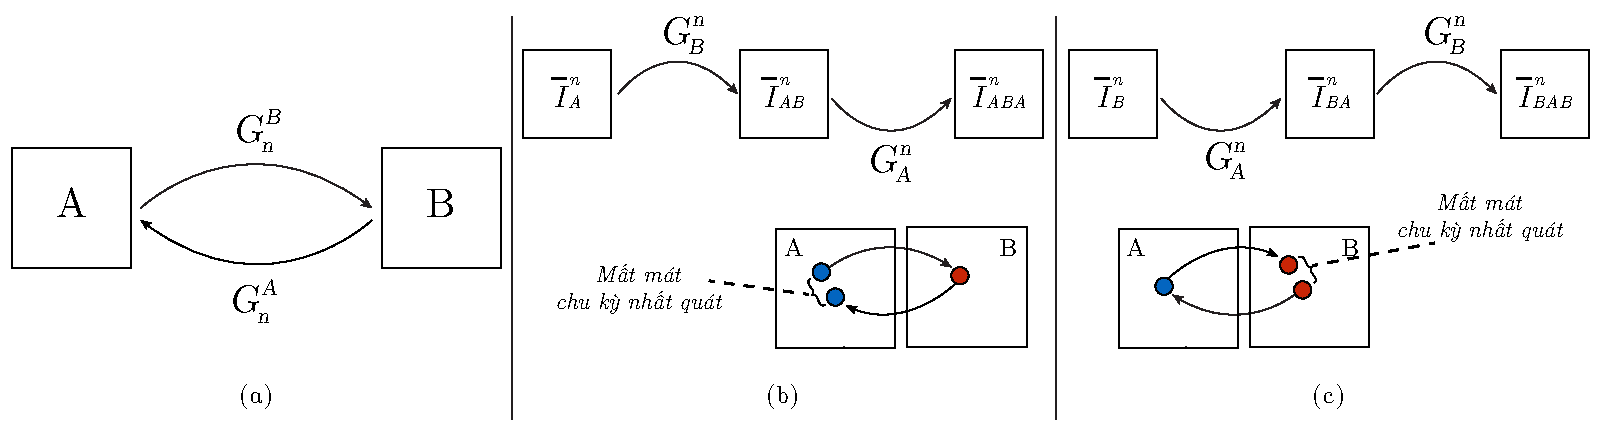
\includegraphics[width=1\textwidth]{img/Cycle-loss.pdf}
	\caption[Mất mát chu kỳ nhất quán]{\blindtext Mất mát chu kỳ nhất quán. \quad Mô hình bao gồm hai ánh xạ $G_n ^A: A \rightarrow B$ và $G_n ^B: B \rightarrow A$, Để đảm bảo ánh xạ chính xác hơn mô hình sử dụng mất mát chu kỳ nhất quán với mục tiêu chuyển đổi hình ảnh từ vùng này sang vùng khác thì kết quả chuyển đổi  phải có khả năng chuyển ngược lại về hình ảnh ban đầu, nên  mất mát chu kỳ nhất quán gồm hai phần: (b) mất mát chu kỳ nhất quán truyền xuôi: $\overline{I}_A \to G_B\left( \overline{I}_A \right) \to G_A\left( {G_B\left( \overline{I}_A \right)} \right) \approx \overline{I}_A$, (c) mất mát chu kỳ nhất quán truyền ngược: $\overline{I}_B \to G_A\left( \overline{I}_B \right) \to G_B\left( {G_A\left( \overline{I}_B \right)} \right) \approx \overline{I}_B$}
	\label{fig:cycle-loss} \vspace{-0.4cm}
\end{figure*}
Vào năm 2017, Zhu cùng cộng sự \cite{zhu2017unpaired} đã đề xuất mất mất chu kỳ nhất quát trong CycleGAN  để giải quyết vấn đề dữ liệu không cùng một cặp. Về mặt lý thuyết, quá trình học dựa trên mất mát đối kháng có thể giúp mô hình tìm ra được hai ánh xạ $G_A$ và $G_B$  tạo được đầu ra tương ứng với miền ảnh mục tiêu $A$ và $B$. Tuy nhiên, để có thể đạt được điều này mô hình cần phải có rất nhiều dữ liệu. Do đó, nếu chỉ dựa vào mỗi hàm học đối kháng thì sẽ khó có thể ánh xạ được $I_A$ sang $I_B$ và chiều ngược lại. 

Để có thể giải quyết bài toán ít dữ liệu, Zhu cùng cộng sự đã chỉ ra rằng ánh xạ mà mô hình học được nên là một chu trình nhất quát (như trong hình \ref{fig:cycle-loss}($b$)). Tức là, mỗi tấm hình $\overline{I}_A \in A$ sẽ được chuyển đổi sang $\overline{I}_{AB} \in B$ và sau đó sẽ được chuyển đổi ngược lại về $\overline{I}_{ABA} \in A$ và  khoảng cách $\overline{I}_A$ và $\overline{I}_{ABA}$ nên được ngắn nhất, $\overline{I}_A \to G_B\left( \overline{I}_A \right) \to G_A\left( {G_B\left( \overline{I}_A \right)} \right) \approx \overline{I}_A$. Tương tự như hình \ref{fig:cycle-loss}($c$), với mỗi hình ảnh $I_B \in B$ sẽ được chuyển đối sang $\overline{I}_{BA} \in A$, và sau đó sẽ được chuyển đổi ngược lại về $\overline{I}_{BAB} \in B$ và khoảng cách $\overline{I}_B$ và $\overline{I}_{BAB}$ nên được ngắn nhất, $\overline{I}_B \to G_A\left( \overline{I}_B \right) \to G_B\left( {G_A\left( \overline{I}_B \right)} \right) \approx \overline{I}_B$. Mô hình sẽ được triển khai mất mát chu kỳ nhất quát cho tất cả các tầng $n=0,1,..., N$ nhằm  làm cho cấu trúc của hai hình ảnh có thể được cân chỉnh phù hợp:
\begin{equation}\label{cycle_loss}
   \mathcal{L}_{cyc_n}\left(G_A ^n, G_B ^n \right) = \left\| {\overline I _A^n - \overline I _{ABA}^n} \right\|_2^2 + \left\| {\overline I _B^n - \overline I _{BAB}^n} \right\|_2^2 
\end{equation}
trong đó $\overline I _{ABA}^n = G_A^n\left( {\overline I _{AB}^n} \right),\overline I _{BAB}^n = G_B^n\left( {\overline I _{BA}^n} \right)$.
%\subsubsection{Mất mát tota vảiation}


Từ phương trình (\ref{adv_loss}), (\ref{rec_loss}) và (\ref{cycle_loss}) hàm mất mát cho mô hình tại tầng $n$ được định nghĩa:
\begin{equation}
   \mathcal{L}_n = \mathop {\min }\limits_{G_A^n,G_B^n} \mathop {\max }\limits_{D_A^n,D_B^n} {\mathcal{L}_{ad{v_n}}} + {\lambda _{rec}}{\mathcal{L}_{re{c_n}}} + {\lambda _{cyc}}{\mathcal{L}_{cy{c_n}}} 
\end{equation}
Trong đó, $\lambda_{rec}$ và $\lambda_{cyc}$ là hai siêu tham số.

\clearpage
\chapter{Kết quả và thảo luận}
\label{result}
\section{Kết quả} %Thẳng thắn nhỉn vào vấn đề, kết quả không tốt, vì lý do nào (A,B,C,D) -> 
Cho trước một video và hình ảnh mục tiêu, mô hình cố gắng chuyển đổi thành một video có chuyển động như video ban đầu nhưng có kiểu dáng, cấu trúc như hình ảnh mục tiêu. Video gốc bao gồm một chuỗi các khung hình $f_1,...,f_k$. Mô hình sẽ chuyển đổi từng khung hình $f_i$ với $i = \overline {1,k} $  của video gốc sang từng khung hình $v_i$ với  $i = \overline {1,k} $ của video đầu ra. Khung hình $v_i$ được định nghĩa như sau:
\begin{equation}
    {v_i} = G_B^N\left( {{f_i} + z} \right)
\end{equation}

Trong đó $z$ là nhiễu Gauss được khởi tạo ngẫu nhiên và giữ cố định xuyên suốt cho tất cả các khung hình $f_i$. Nhiễu $z$ giúp cho các khung hình tạo ra liên tục về mặt thời gian, kết quả được trình bày trong hình \ref{fig:result}.
\begin{table}[b]
\centering
\captionof{table}{So sánh kiến trúc giữa nghiên cứu này và Benaim cùng cộng sự}
\resizebox{\textwidth}{!}
{%
\begin{tabular}{@{}lccccc@{}}
\toprule
\multicolumn{1}{c}{Mô hình} & \begin{tabular}[c]{@{}c@{}}Số lượng\\ bộ sinh\end{tabular} & \begin{tabular}[c]{@{}c@{}}Số lượng\\ bộ phân biệt\end{tabular} &  Số tầng & \begin{tabular}[c]{@{}c@{}}Số lượng\\ tham số\end{tabular} \\ \midrule
Nghiên cứu này                         & 2                                                            & 2                                                                                                                & 6       & $\sim1,320,000$                                            \\
Benaim và cộng sự \cite{benaim2020structuralanalogy}                      & 2                                                            & 2                                                                                                            & 10      & $\sim2,600,000$                                            \\ \bottomrule
\end{tabular}%
}
\label{parameter-model}
\end{table}
\begin{figure*}[t]
\vspace{-0.5cm}
	\centering
	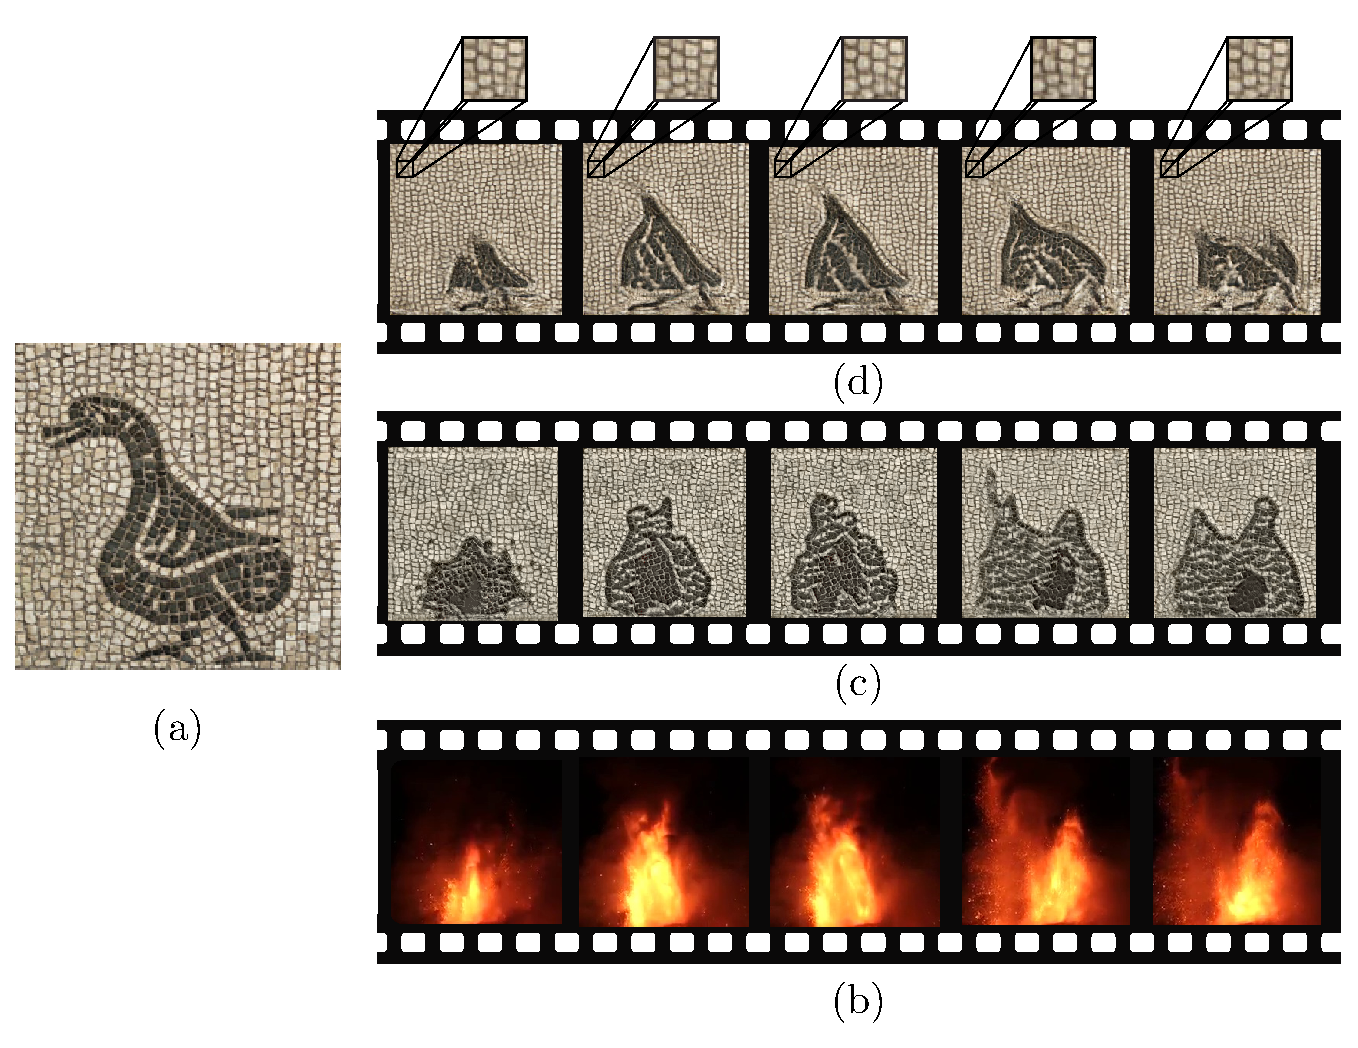
\includegraphics[width=1\textwidth]{img/result.pdf}
	\caption[Video chuyển đổi]{\blindtext Video chuyển đổi. \quad Mô hình chuyển đổi giữa video gốc là video núi lửa và hình ảnh mục tiêu là hình ảnh con vịt đá. (a) Hình ảnh mục tiêu. (b) Video gốc với các khung hình đầu vào $f_i$. (c)  Kết quả các khung hình được chuyển đổi bằng mô hình của Benaim cùng nhóm cộng sự \cite{benaim2020structuralanalogy}. (d) Kết quả của các khung hình được chuyển đổi $v_i$ bằng mô hình trong nghiên cứu này. Hình ảnh phóng to của (d) là một phần trong các khung hình $v_i$ để thấy được các khung hình chuyển đổi xuyên suốt đều không có chuyển động.}
	\label{fig:result} \vspace{-0.4cm}
\end{figure*}
%Nói về số lượng parameters
Nhờ vào cấu trúc đa tầng và các phương pháp thay đổi trên (được đề cập ở chương \ref{our-method}) đã giúp cho mô hình giảm được số lượng tham số  khoảng $50.77\%$ (xem bảng \ref{parameter-model}). Mô hình được huấn luyện với kỹ thuật tối ưu  Adam \cite{kingma2014adam}, tốc độ học ban đầu là $0.0005$, cứ sau mỗi tầng mô hình sẽ giảm tốc độ học xuống 10 lần. Tại bất kỳ một tầng $n$,  thay vì  sử dụng cùng một tốc độ học cho tất cả các tầng $\left( n, n-1, n -2, ... \right)$ thì dùng tốc độ học nhỏ hơn cho những tầng thấp hơn  $\left(  n-1, n -2, ... \right)$ sẽ giúp giảm được hiện tượng quá khớp. Do đó,  tốc độ học $\eta$ với hệ số $\delta$ sẽ thay đổi ngày càng chậm. Cụ thể, tại mỗi tầng $n$, mô hình sẽ huấn luyện với tốc độ học là ${\delta}\eta $. Ví dụ, tầng thứ $n-1$ sẽ được huấn luyện với tốc độ học ${\delta ^1}\eta $ tầng thứ $n-2$ sẽ huấn luyện với tốc độ học ${\delta ^2}\eta $. Trong nghiên cứu này, cho thấy được là $\delta  = 0.1$ là điểm cân bằng giữa chất lượng hình ảnh và độ đa dạng của hình ảnh tạo ra.

Mô hình được huấn luyện 3000 vòng lặp tại mỗi tầng, có tất cả 6 tầng. Các tham số trọng số của mô hình được cài đặt như mô hình của Benaim và cộng sự \cite{benaim2020structuralanalogy} $\lambda_{pen} = 0.1 $, $\lambda_{rec} = 1$ và $\lambda_{cyc} = 10$. Kết quả được trình bày trong hình \ref{fig:result}. Khi kết quả không tốt, mô hình được thay đổi bằng cách tăng $\lambda_{cyc} = 20$ vì để giúp cho việc ánh xạ qua lại giữa hai miền ảnh tốt hơn. Tuy nhiên, điều này dẫn đến quá trình huấn luyện mô hình không thể hội tụ hoặc hội tụ với kết quả cũng không tốt. Nghiên cứu này đã thử trên rất bộ siêu tham số khác nhau nhưng kết quả đều không tốt.



%Nhìn thẳng vào vấn đề
Các khung hình được tạo ra vẫn giữ được tính liên tục về mặt thời gian, tức là những vùng cần chuyển động thì mới chuyển động còn những vùng nên cố định thì mô hình vẫn giữ được (xem phần phóng to của hình \ref{fig:result} (d)). Các thông tin về hoa văn và họa tiết của hình ảnh \ref{fig:result} (a) được mô hình học rất tốt. Tuy nhiên, khi chuyển đổi sang các khung hình thì kết quả mô hình tạo ra hoàn toàn không tốt. Mô hình không thể chuyển đổi được cấu trúc ngọn lửa theo được kiểu dáng của hình \ref{fig:result} (a). Có thể thấy các viền của ngọn lửa không được mượt (xem  hình \ref{fig:result} (d)), các khung hình được tạo ra vẫn còn sót lại cấu trúc tổng quát của hình mục tiêu \ref{fig:result} (a) mà không thể chuyển đổi hoàn toàn. Trong khi kết quả của mô hình trong nghiên cứu Benaim và cộng sự  (xem  hình \ref{fig:result} (c)) thật sự rất tốt, mô hình của nhóm tác giả đã học được cả cấu trúc của ngọn lửa dưới kiểu dáng của tấm hình mục tiêu. 

%Tại sao lại xảy ra những điều đó

%Tại sao lại suy nghĩ như vậy?
\clearpage
\section{Thảo luận}
Mô hình ConSinGAN giảm thời gian huấn luyện SinGAN xuống còn $20-30\text{ phút}$ và nghiên cứu của Benaim và cộng sự ứng dụng được SinGAN trong bài toán chuyển đổi hình ảnh sang hình ảnh.
Do đó, khi kết hợp 2 mô hình lại với nhau, với mong muốn mô hình mới sẽ có thể tạo ra được kết quả tốt và vẫn có thể giữ lại những điểm mạnh về thời gian huấn luyện cũng như khả năng ứng dụng của mô hình. Mô hình trong nghiên cứu này đã giảm được thời gian huấn luyện đáng kể.
Tuy nhiên, kết quả tạo ra lại đi ngược lại với những  điều  mong đợi từ ban đầu. Dưới đây là một số nguyên nhân có thễ dẫn đến việc tạo kết quả trong mô hình không tốt:
\begin{itemize}
    \item Cấu trúc mô hình đã được rút gọn dẫn đến việc học các thông tin trở nên vừa đủ làm cho mô hình không thể có nhiều thông tin để chuyển đổi.
    \item Trong quá trình thay đổi kích thước hình ảnh, độ phân giải chủ yếu là độ phân giải thấp, dẫn đến  mô hình  không đủ tầng để có thể học được các đặc trưng khác của hình ảnh.
    \item Bằng cách chỉ truyền vào mô hình các đặc trưng được học ở tầng trước đã làm cho mô hình học rất tốt cấu trúc tổng quát của tấm hình gốc  nên dẫn đến việc mô hình chỉ có thể tạo ra được các kết quả giống với tấm hình gốc ban đầu (có thể nhìn nhận đây là hiện tượng sụp đổ mô hình).
    \item Tốc độ huấn luyện bộ sinh và bộ phân biệt trên hai miền ảnh là khác nhau, nghĩa là, quá trình huấn luyện $G_A$, $D_A$ trên miền ảnh $A$ đã hội tụ nhưng quá trình huấn luyện $G_B$, $D_B$ trên miền ảnh $B$ vẫn chưa hội tụ mà  lại vội đưa kết quả qua tầng kế tiếp. Điều này, có thể hiểu như lỗi chồng lỗi khiến cho mô hình bị thiên về một miền ảnh, còn miền ảnh kia thì không học thêm được thông tin gì.
\end{itemize}

\clearpage
\chapter{Kết luận}
Tính đến hiện tại, số lượng các mô hình có thể giải quyết được bài toán chuyển đổi hình ảnh mà huấn luyện trên một cặp dữ liệu là rất ít \cite{benaim2020structuralanalogy,lin2020tuigan}.
Trong khuôn khổ của khóa luận tốt nghiệp, nghiên cứu này cố gắng đưa ra hướng giải quyết bài toán chuyển đổi hình ảnh sang hình ảnh với thời gian huấn luyện ngắn nhất, nhưng kết quả mang lại không tốt. Vì để huấn luyện được mô hình GAN thông thường  cần rất nhiều dữ liệu, chưa kể đến việc các mô hình chuyển đổi hình ảnh thường sẽ huấn luyện trên cả hai bộ sinh và hai bộ phân biệt nên sẽ rất dễ dấn đến các hiện tượng như  sụp đổ mô hình, dưới khớp, quá khớp,... Đồng thời, các mô hình GAN rất dễ nhạy cảm với các siêu tham số.
Tóm lại, cách kết hợp trong mô hình của nghiên cứu này đưa ra là không phù hợp. Tuy nhiên, điều này đã làm tiền đề giúp cho các nghiên cứu sau có thể tránh đi theo vết xe đổ, nhờ đó sẽ không gây lãng phí về thời gian cũng như công sức vào hướng đi này.

\clearpage

\chapter{Đề nghị nghiên cứu thêm}
Với những kết quả như được trình bày trong chương \ref{result} đã tạo ra  động lực để  có thể tiếp tục nghiên cứu phát triển mô hình này. Có thể nói, trong tương lai mô hình đã tránh được một trong các hướng đi thất bại. Trong thời gian sắp tới, nghiên cứu vẫn tiếp tục giải quyết bài toán chuyển đổi hình ảnh  trên một cặp hình ảnh duy nhất với thời gian huấn luyện ngắn bằng cách đưa vào một video chứ không đơn thuần là một tấm ảnh như nghiên cứu này. Việc đưa vào một video có thể giúp cho mô hình học được nhiều thông tin hơn như \word{dòng quang}{optical flow}của một video. Đồng thời,  có thể thử sử dụng phương pháp thay đổi kích thước hình ảnh như mô hình \cite{benaim2020structuralanalogy}  để giúp cho mô hình có thể học được nhiều tầng hơn. Ngoài ra, còn có thể sử dụng thêm các hàm mất mát khác để làm cho mô hình phức tạp hơn nhằm học được các cấu trúc tổng quát của video .
Hy vọng rằng, mô hình sẽ không chỉ dừng lại giải quyết bài chuyển đổi hình ảnh sang hình ảnh mà còn có thể mở rộng thêm các ứng dụng khác cho mô hình như siêu phân giải hình ảnh, hòa trộn ảnh, chỉnh sửa hình ảnh,...


\clearpage
\printbibliography[title={Tài liệu tham khảo}]
\end{document}
